 
\begin{enumerate}[label=\thesection.\arabic*.,ref=\thesection.\theenumi]
\numberwithin{equation}{enumi}

\item Sketch the Bode Magnitude and Phase plot for the following system. Also compute the gain margin and the phase margin.
\begin{align}
G\brak{s} &= \frac{10}{s\brak{1+0.5s}\brak{1+.01s}}
\label{eq:ee18btech11048_2}
\end{align}
\\
\solution 
The system is defined as follows:
\begin{align}
G\brak{s} &= \frac{10}{s\brak{1+0.5s}\brak{1+.01s}}
\end{align}
\begin{table}[!ht]
\centering
\input{./tables/ee18btech11048_tebles.tex}
\caption{Zeros and Poles}
\label{table:ee18btech11048}
\end{table}\\
The magnitude and phase plot are as follows: Fig\ref{fig:ee18btech11048} 
\begin{figure}[!h]
\centering
  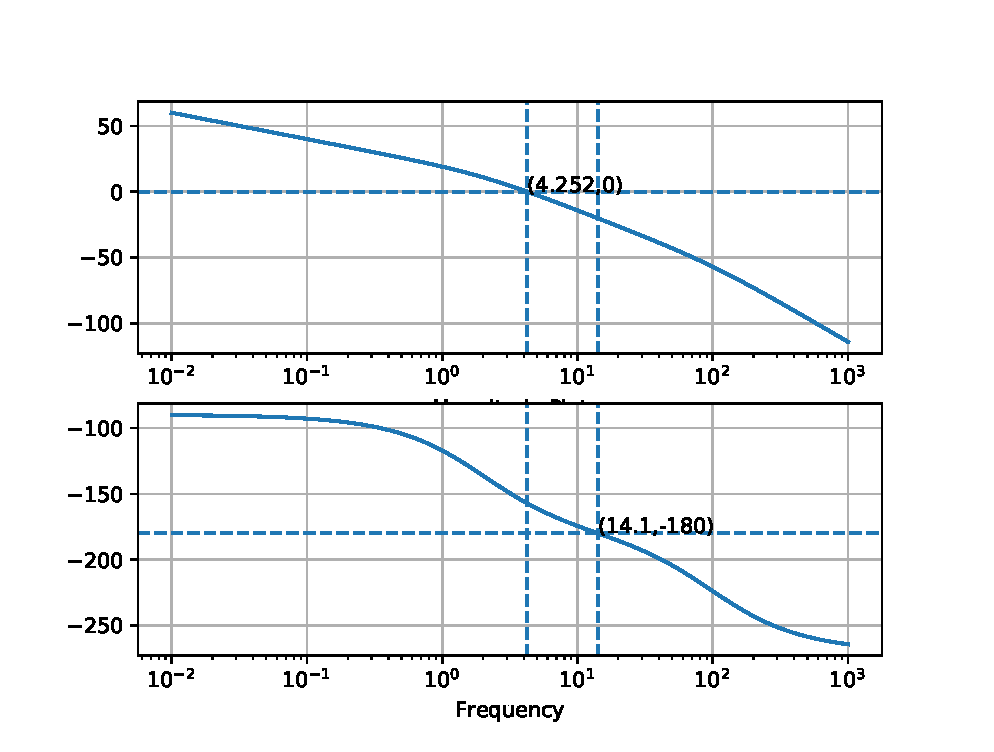
\includegraphics[width=\columnwidth]{./figs/ee18btech11048.eps}
  \caption{Graphs}
  \label{fig:ee18btech11048}
\end{figure}

The python code to obtain the graphs:

\begin{lstlisting}
codes/ee18btech11048.py
\end{lstlisting}

\item {\em Gain} and {\em Phase} of Transfer Function 
\begin{align}
G\brak{j\omega} &= \frac{10}{j\omega\brak{1+0.5j\omega}\brak{1+.01j\omega}}
\end{align}
Gain:
\begin{align}
    \frac{100}{\omega\sqrt{\brak{0.5\omega}^2+1}\sqrt{\brak{0.01\omega}^2+1}}
\label{eq:ee18btech11048_2}
\end{align}{}
Phase:
\begin{multline}
\tan^{-1} \brak{0}-\tan^{-1} \brak{\frac{\omega}{0}} - \tan^{-1} \brak{\frac{\omega}{2}}- \\\tan^{-1} \brak{\frac{\omega}{100}} 
\label{eq:ee18btech11048_3}
\end{multline}
\item Finding the Phase Margin\brak {PM}
\begin{align}
{\em PM} = \angle G(\j\omega_{gc}) + 180\degree \\
\omega_{gc}=\text{Gain Crossover Frequency}\\
\text{At }  \omega_{gc} \left| G\brak{s}\right|  = 1
\end{align}
\solution
\begin{align}
    \frac{100}{\omega_{gc}\sqrt{\brak{0.5\omega_{gc}}^2+1}\sqrt{\brak{0.01\omega_{gc}}^2+1}} &= 1
\label{eq:ee18btech11048_2}
\end{align}{}
Solving Eq. \eqref{eq:ee18btech11048_2} {\em or} from Fig \ref{fig:ee18btech11048} :

\begin{align}
\implies
\omega_{gc} &= 4.25  \\
\angle G\brak{\j\omega_{gc}} &= -157.2 \\
\implies
PM &= 22.8 
\end{align}

\item Finding the Gain Margin \brak{GM}\\
\begin{align}
{\em GM} = 0 -G(\j\omega_{pc}) db \\
\omega_{pc}=\text{Phase Crossover Frequency}\\
\text{At }  \omega_{pc} \angle G\brak{s}  = -180\degree
\end{align}
 \\
\solution

\begin{multline}
\tan^{-1} \brak{0}-\tan^{-1} \brak{\frac{\omega_{pc}}{0}} - \tan^{-1} \brak{\frac{\omega_{pc}}{2}}- \\\tan^{-1} \brak{\frac{\omega_{pc}}{100}} = -180\degree
\label{eq:ee18btech11048_3}
\end{multline}
Solving Eq. \eqref{eq:ee18btech11048_3} {\em or} from Fig \ref{fig:ee18btech11048} :

\begin{align}
\implies
\omega_{pc} &=  14.1 \\
 -\text{G}(\j\omega_{pc}) db &= -20.2 db \\
\implies
GM &= 20.2 db
\end{align}

\end{enumerate}
